\documentclass{jsarticle}
\usepackage[dvipdfmx]{graphicx}
\usepackage{listings,jlisting}
\lstset{%
  language={C},
  basicstyle={\small\ttfamily},%
  identifierstyle={\small},%
  commentstyle={\small\itshape},%
  keywordstyle={\small\bfseries},%
  ndkeywordstyle={\small},%
  stringstyle={\small\ttfamily},
  frame={tb},
  breaklines=false,
  columns=[l]{fullflexible},%
  numbers=left,%
  xrightmargin=0zw,%
  xleftmargin=3zw,%
  numberstyle={\scriptsize},%
  stepnumber=1,
  numbersep=1zw,%
  lineskip=-0.5ex%
}

\begin{document}

\title{画像工学 レポート\\ \vspace{1cm}― 画像の平滑化とエッジ抽出 ―\vspace{2cm}}
\author{IE5 (9) 片岡 駿之介 \vspace{1cm}}
\maketitle

\newpage

\section{課題}

画像処理の中には,画像内に含まれる雑音を除去したり,画像の持つ特徴を抽出したりといった目的で,画像に対してフィルタリングと呼ばれる処理を行うことがある.本課題では,フィルタリングの中でも「平滑化」と「エッジ抽出」に着目している.「平滑化」は,主に画像中に含まれているインパルスノイズを取り除く目的で使用される.「エッジ抽出」は,画像中の特徴を知りたい時に画像中のエッジのみを取り出す目的で使用される.\\
今回,課題において「平滑化」については「加重平均フィルタ」と「メディアンフィルタ」,「エッジ抽出」に関しては「ラプラシアンフィルタ」を実装し,それぞれの出力結果を確かめる.

\section{処理の流れ}

今回の演習では,PGMファイルを以下の手順で処理していくこととした.
\begin{enumerate}
  \item 入力されたコマンドが正しいかチェック(正しくない場合はUsageを表示して終了)
  \item コマンドで指定されたPGMファイルを読み込む
  \item 読み込んだPGMファイルのヘッダ解析
  \item ヘッダが正しければ画素値を2次元配列に取り込む
  \item コマンドで指定されたフィルタリング処理を施す
  \item コマンドで指定されたファイルへ画像を出力する
\end{enumerate}

この処理によって得られたPGMファイルをImageMagickを用いて表示し,処理前後で画像がどのように変化するかを比較検討する.\\
なお,縁に関しては元の画像の画素値を代入している.
\newpage

\section{ソースリスト}

\begin{lstlisting}[caption=filter.c,label=ほげ]
  #include <stdio.h>
  #include <stdlib.h>
  #include <string.h>
  #include <ctype.h>

  FILE *fp;

  int width;
  int height;
  int max_value;
  int status;
  char buffer[128];

  void image_open(char *file_name) {
    if ((fp = fopen(file_name, "r")) == NULL) {
  		printf("file open error!!\n");
  		exit(-1);	/* (3)エラーの場合は通常、異常終了する */
  	}
  }

  int main(int argc,char *argv[]) {

    /* 入力コマンドのチェック */
    if(argc != 5) {
      printf("Usage : ./filter <filter type> <kernel size> <input pgm filename> <output pgm filename>\n");
      exit(0);
    } else if (argc == 5) {
      image_open(argv[3]);
      printf("filter type : %s\n", argv[1]);
      printf("kernel size : %s\n", argv[2]);
    }

    /* ヘッダ取得部 */
    int ch;

    while (status < 3) {
      ch = getc(fp);

      if(ch == '#') { // コメントのスキップ
        while (( ch = getc(fp)) != '\n')
          break;
      }

      if(ch == 'P') { // マジックナンバーのチェック
        if(getc(fp) != '5') {
          printf("Magic Number is wrong.\n");
          break;
        } else {
          // printf("Magic Number is P5\n");
        }
      }

      if(isdigit((unsigned char)ch)) { // 数値取得部
        buffer[0] = ch;
        int i=1;
        while(1) {
            char c = getc(fp);
            if(isdigit((unsigned char)c)) {
              buffer[i]=c;
              i++;
            } else
              break;
        }
        buffer[i] = '\0';

        switch (status) {
          case 0: // width取得部
            width = atoi(buffer);
            printf("width=%d\n", width);
            break;
          case 1: // height取得部
            height = atoi(buffer);
            printf("height=%d\n", height);
            break;
          case 2: // max_value取得部
            max_value = atoi(buffer);
            printf("max_value=%d\n", max_value);
            break;
        }
        status++; // 次のステータスへ
      }
    }

    /* 画素値取得部 */
    int image[width][height];

    for(int i = 0; i < height; i++) {
      for(int j = 0; j < width; j++) {
        image[j][i] = (int)getc(fp);
      }
    }

    /* フィルタ処理部 */

    int kernel_size = atoi(argv[2]);
    int output_image[width][height];

    for(int i=0; i < height; i++) {
      for(int j=0; j < width; j++) {
        output_image[j][i] = image[j][i];
      }
    }

    if(strcmp(argv[1], "average") == 0) { //加重平均フィルタ

      int padding = ((kernel_size - 1)/2);
      printf("padding:%d\n", padding);

      int i, j;

      for(i=padding; i < (height-padding); i++) {
        for(j=padding; j < (width-padding); j++) {
          int sum = 0;

          for(int k = -padding; k <= padding; k++) {
            for(int l = -padding; l <= padding; l++) {
              sum += image[j+k][i+l];
            }
          }
          output_image[j][i] = (int)(sum / (kernel_size * kernel_size));
        }
      }

    } else if(strcmp(argv[1], "median") == 0) { //メディアンフィルタ
      int padding = ((kernel_size - 1)/2);
      printf("padding:%d\n", padding);

      int i, j;

      for(i=padding; i < (height-padding); i++) {
        for(j=padding; j < (width-padding); j++) {
          int sum = 0;
          int median_array[kernel_size * kernel_size];
          int median_cnt = 0;

          for(int m = 0; m < kernel_size * kernel_size; m++)
            median_array[m] = 0;

          for(int k = -padding; k <= padding; k++) {
            for(int l = -padding; l <= padding; l++) {
              median_array[median_cnt] = image[j+k][i+l];
              median_cnt++;
            }
          }

          for(int m = 0; m < (kernel_size * kernel_size); m++) {
            for(int n = 0; n < (kernel_size * kernel_size); n++) {
                  if (median_array[n+1] < median_array[n]) {
                      int buf = median_array[n+1];
                      median_array[n+1] = median_array[n];
                      median_array[n] = buf;
                  }
              }
          }

          output_image[j][i] = (int)median_array[(kernel_size * kernel_size) / 2];
        }
      }
    } else if(strcmp(argv[1], "laplacian") == 0) { //ラプラシアンフィルタ
      if(kernel_size != 3) {
        printf("ラプラシアンフィルタを適用する場合はカーネルサイズを3にしてください\n");
        exit(0);
      }

      int padding = ((kernel_size - 1)/2);
      printf("padding:%d\n", padding);
      int laplacian[3][3] = {{1, 1, 1}, {1, -8, 1}, {1, 1, 1}};
      int i, j;

      for(i=padding; i < (height-padding); i++) {
        for(j=padding; j < (width-padding); j++) {
          int sum = 0;

          for(int k = -padding; k <= padding; k++) {
            for(int l = -padding; l <= padding; l++) {
              sum += (image[j+k][i+l] * laplacian[k+padding][l+padding]);
            }
          }
          if(sum < 0)
            output_image[j][i] = 0;
          else if(sum > 255)
            output_image[j][i] = 255;
          else
            output_image[j][i] = (int)sum;
        }
      }
    }

    /* 画像出力部 */

    FILE *output = fopen(argv[4], "wb");
    char header[30];
    sprintf(header, "P5 %d %d %d\n", width, height, max_value);
    fputs(header, output);
    for(int i = 0; i < height; i++) {
      for(int j = 0; j < width; j++) {
        fputc((char)output_image[j][i], output);
      }
    }
    printf("image was output.\n");
    fclose(output);
  }


\end{lstlisting}

\newpage

\section{結果}
結果の確認には,配布された「town.pgm」を用いた.\\
以下に,それぞれのフィルタを適用した場合の適用前後の比較画像を示す.

\begin{figure}[htbp]
 \begin{minipage}{0.5\hsize}
  \begin{center}
   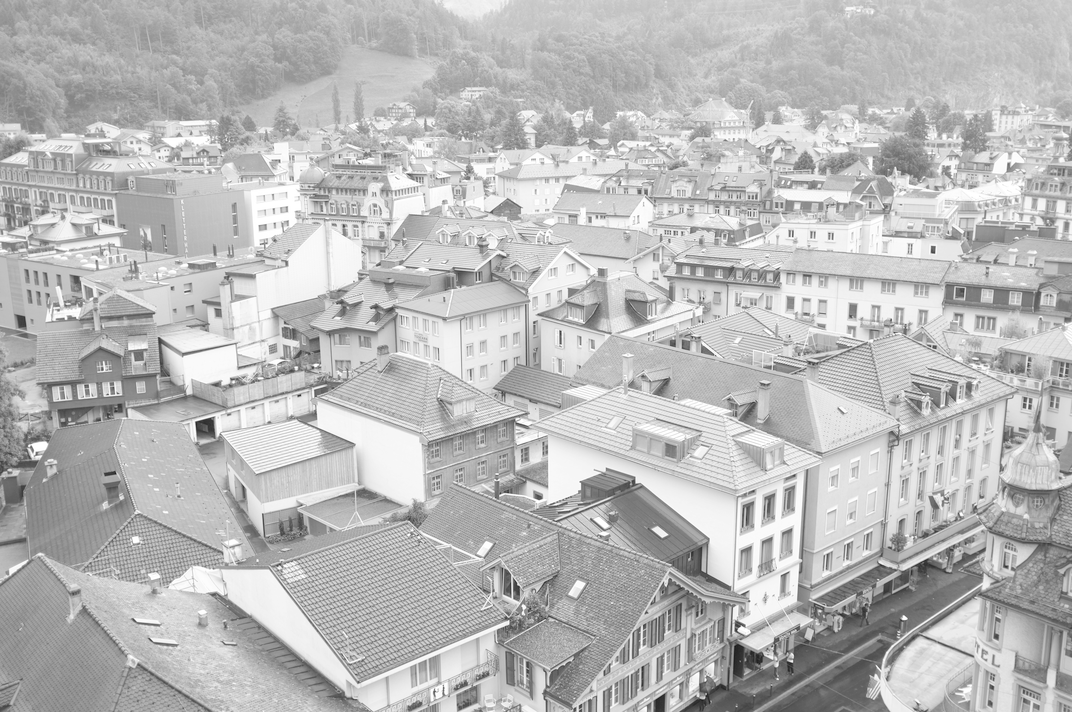
\includegraphics[width=70mm]{town.png}
  \end{center}
  \caption{適用前}
  \label{fig:one}
 \end{minipage}
 \begin{minipage}{0.5\hsize}
  \begin{center}
   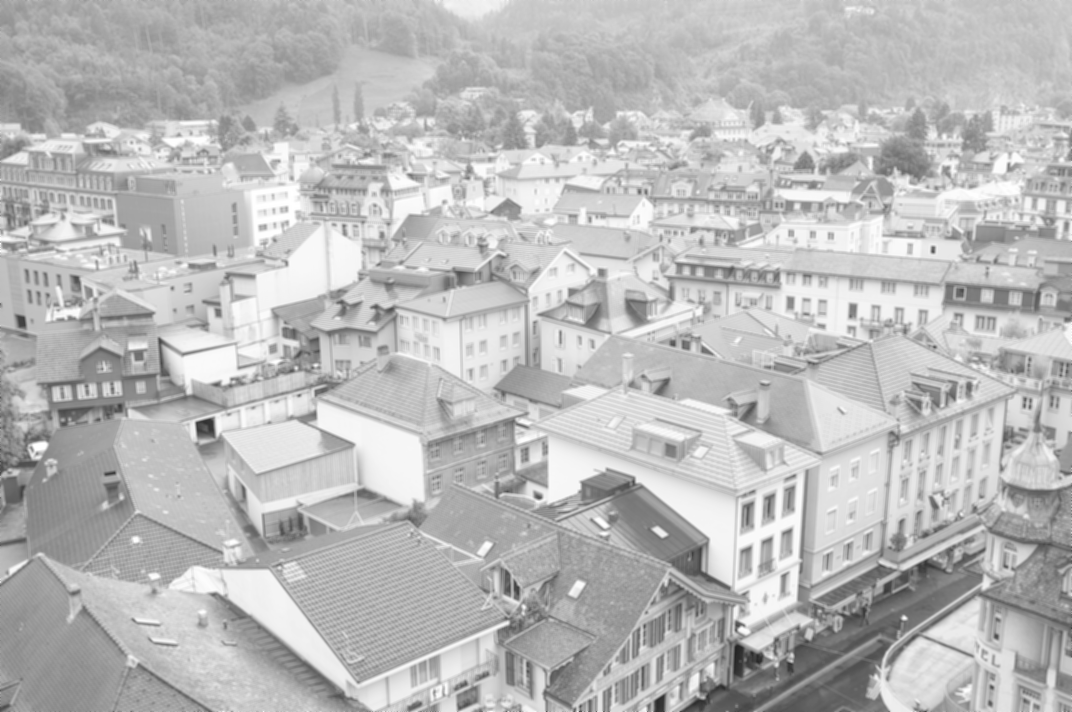
\includegraphics[width=70mm]{output_ave_3.png}
  \end{center}
  \caption{適用後}
  \label{fig:two}
 \end{minipage}
 \caption{加重平均フィルタを適用(カーネルサイズ:3)}
\end{figure}

\begin{figure}[htbp]
 \begin{minipage}{0.5\hsize}
  \begin{center}
   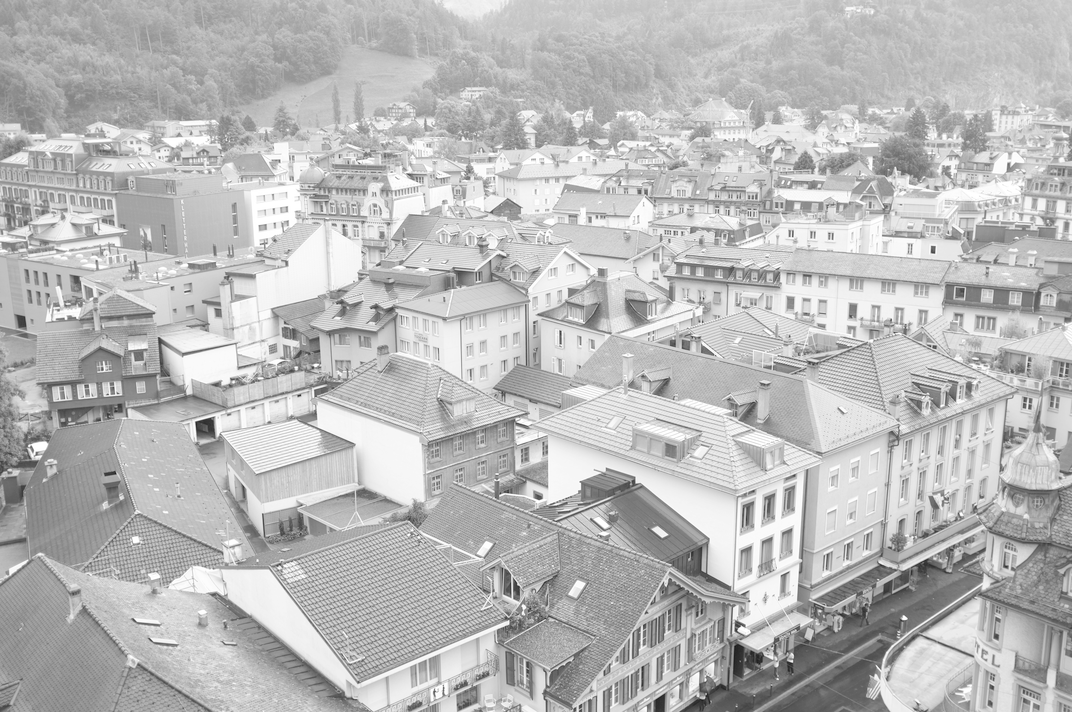
\includegraphics[width=70mm]{town.png}
  \end{center}
  \caption{適用前}
  \label{fig:one}
 \end{minipage}
 \begin{minipage}{0.5\hsize}
  \begin{center}
   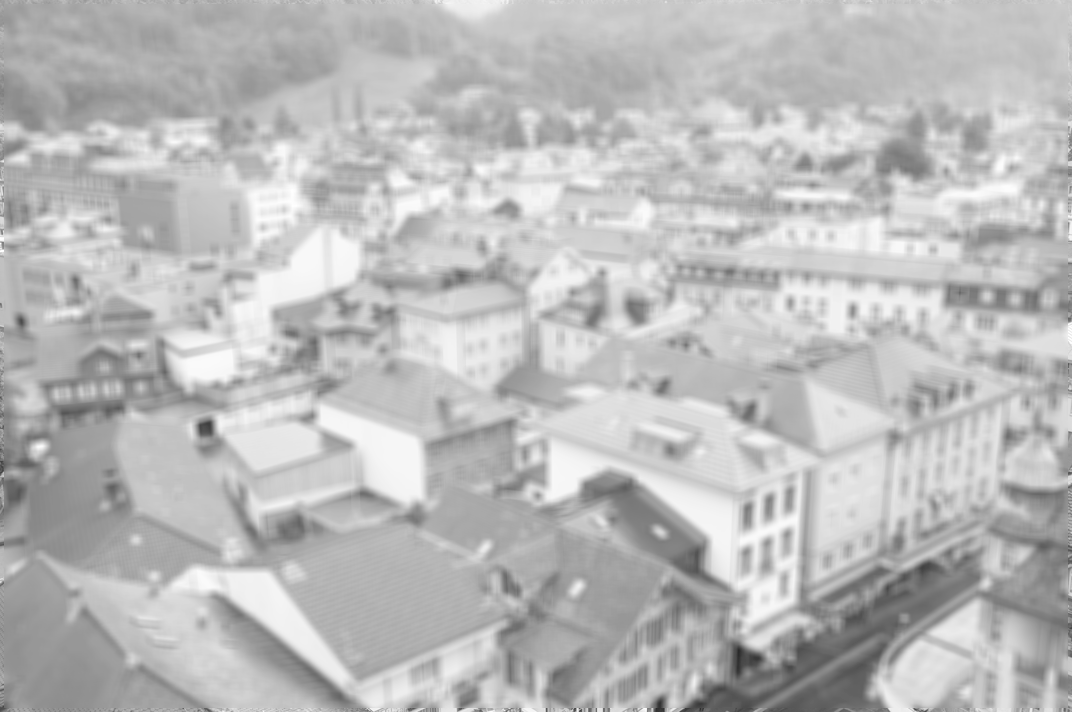
\includegraphics[width=70mm]{output_ave_9.png}
  \end{center}
  \caption{適用後}
  \label{fig:two}
 \end{minipage}
 \caption{加重平均フィルタを適用(カーネルサイズ:9)}
\end{figure}

\begin{figure}[htbp]
 \begin{minipage}{0.5\hsize}
  \begin{center}
   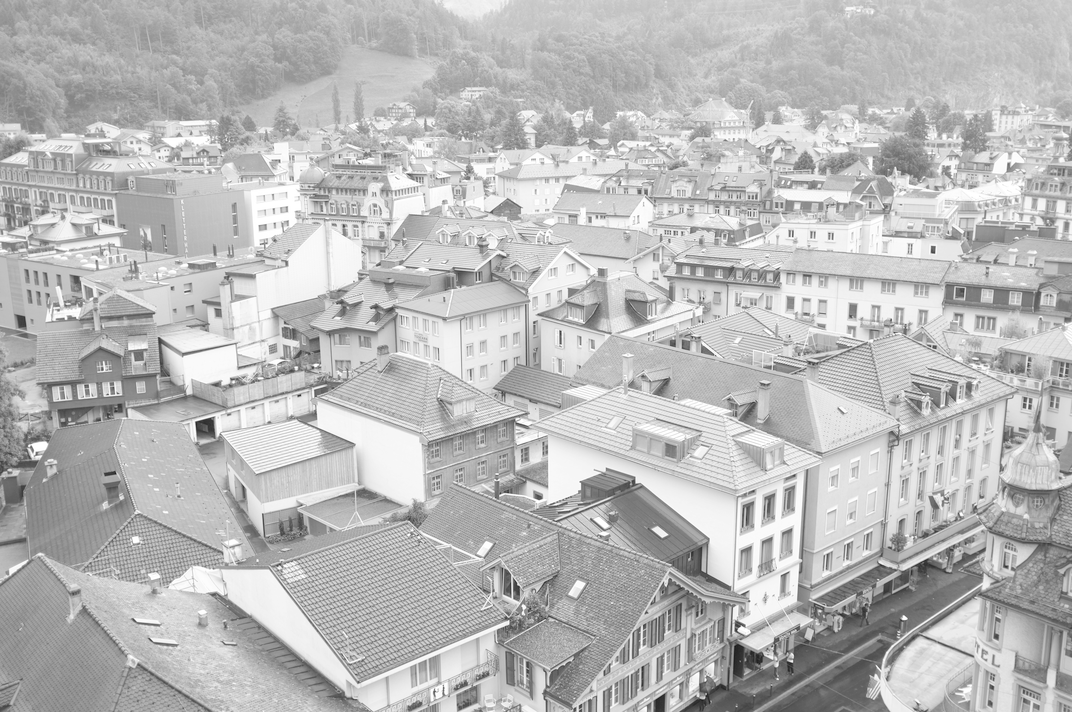
\includegraphics[width=70mm]{town.png}
  \end{center}
  \caption{適用前}
  \label{fig:one}
 \end{minipage}
 \begin{minipage}{0.5\hsize}
  \begin{center}
   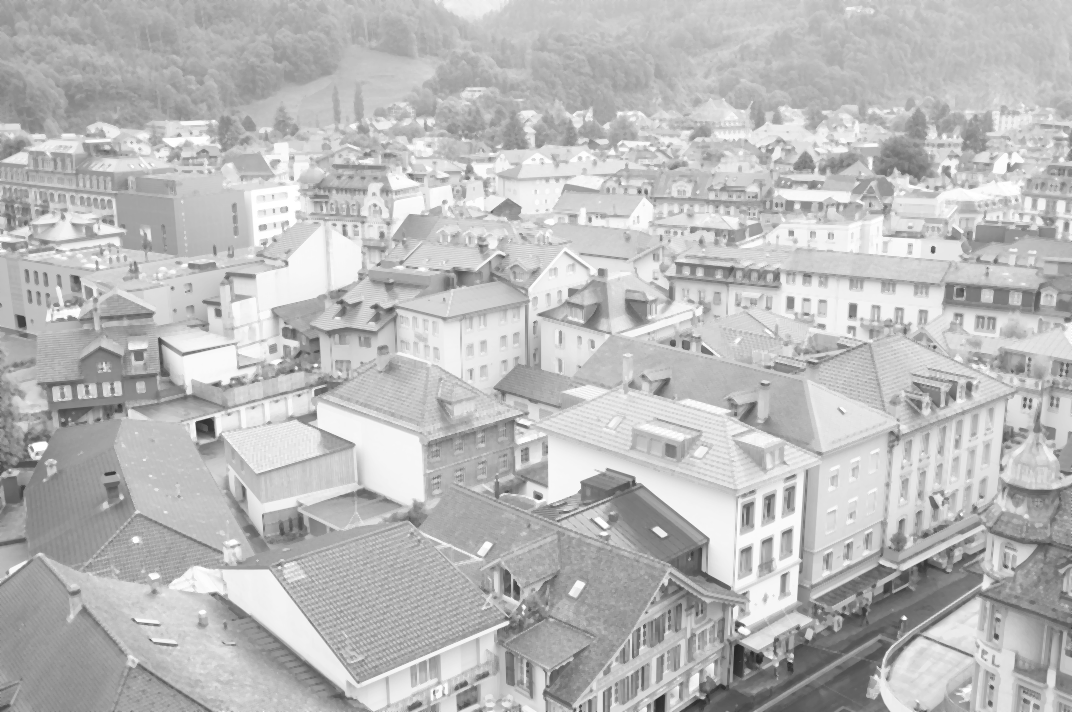
\includegraphics[width=70mm]{output_median_3.png}
  \end{center}
  \caption{適用後}
  \label{fig:two}
 \end{minipage}
 \caption{メディアンフィルタを適用(カーネルサイズ:3)}
\end{figure}


\begin{figure}[htbp]
 \begin{minipage}{0.5\hsize}
  \begin{center}
   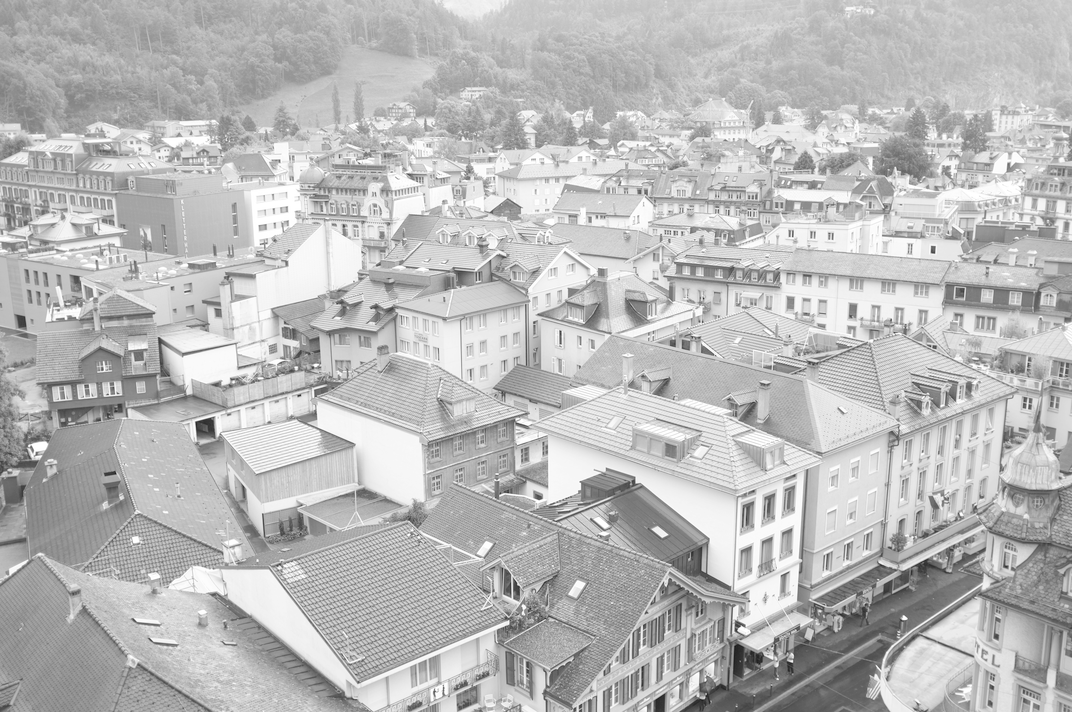
\includegraphics[width=70mm]{town.png}
  \end{center}
  \caption{適用前}
  \label{fig:one}
 \end{minipage}
 \begin{minipage}{0.5\hsize}
  \begin{center}
   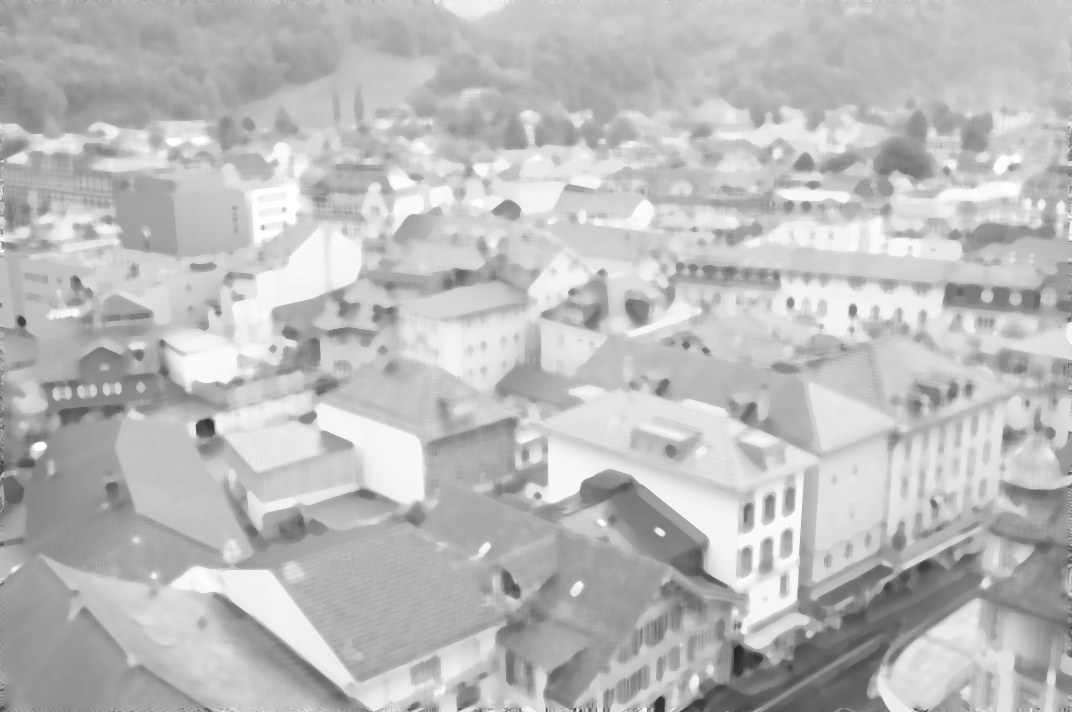
\includegraphics[width=70mm]{output_median_9.png}
  \end{center}
  \caption{適用後}
  \label{fig:two}
 \end{minipage}
 \caption{メディアンフィルタを適用(カーネルサイズ:9)}
\end{figure}

\begin{figure}[htbp]
 \begin{minipage}{0.5\hsize}
  \begin{center}
   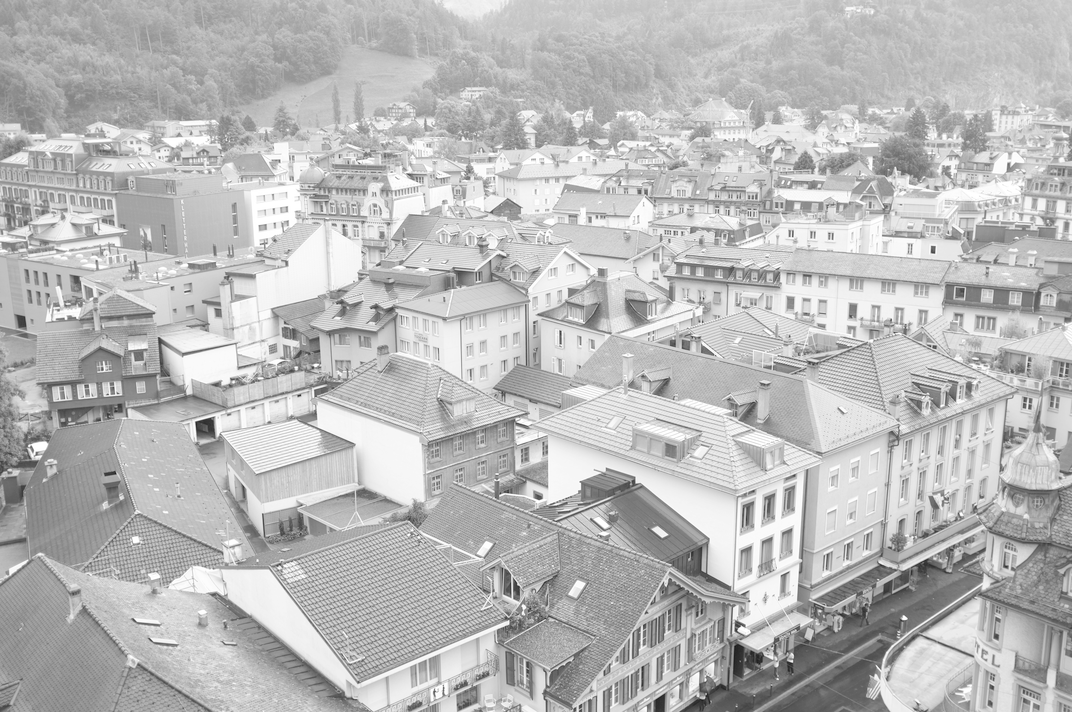
\includegraphics[width=70mm]{town.png}
  \end{center}
  \caption{適用前}
  \label{fig:one}
 \end{minipage}
 \begin{minipage}{0.5\hsize}
  \begin{center}
   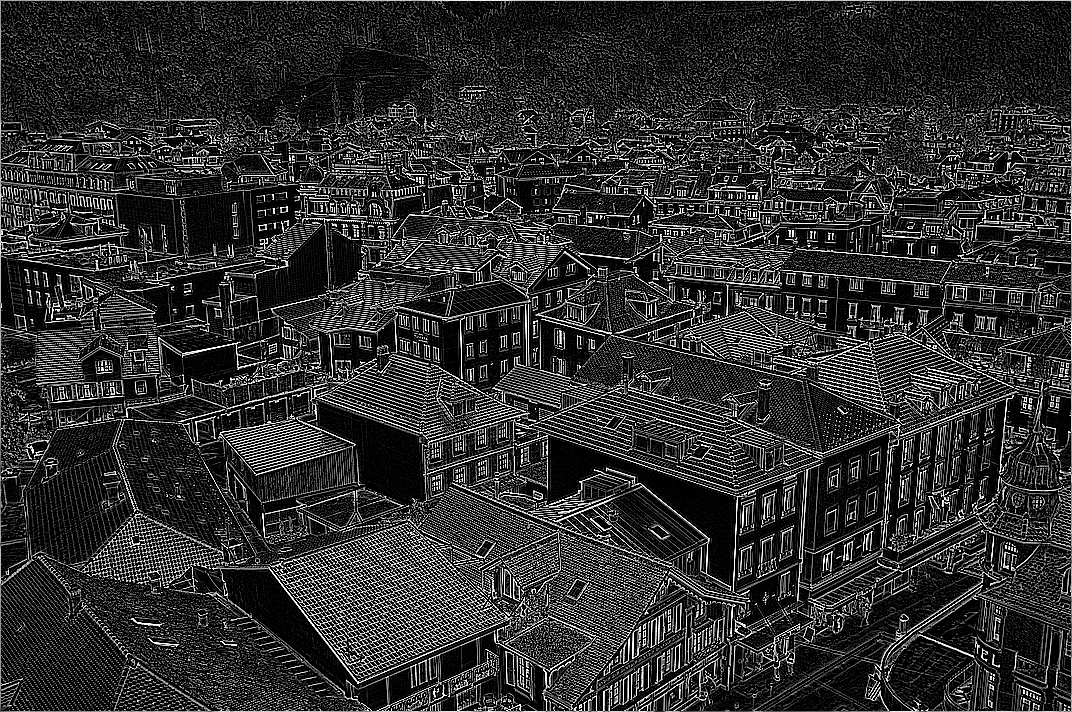
\includegraphics[width=70mm]{output_laplacian.png}
  \end{center}
  \caption{適用後}
  \label{fig:two}
 \end{minipage}
 \caption{ラプラシアンフィルタを適用(カーネルサイズ:3)}
\end{figure}

\newpage

また,今回はノイズ除去の効果を評価するために,メディアンフィルタを用いて,それぞれカーネルサイズが3と9でのノイズ除去の効果を比較した.
ノイズ除去効果の確認には,Photoshopにてノイズを10%載せた「town\_noise.pgm」を使用した.

\begin{figure}[htbp]
 \begin{minipage}{0.5\hsize}
  \begin{center}
   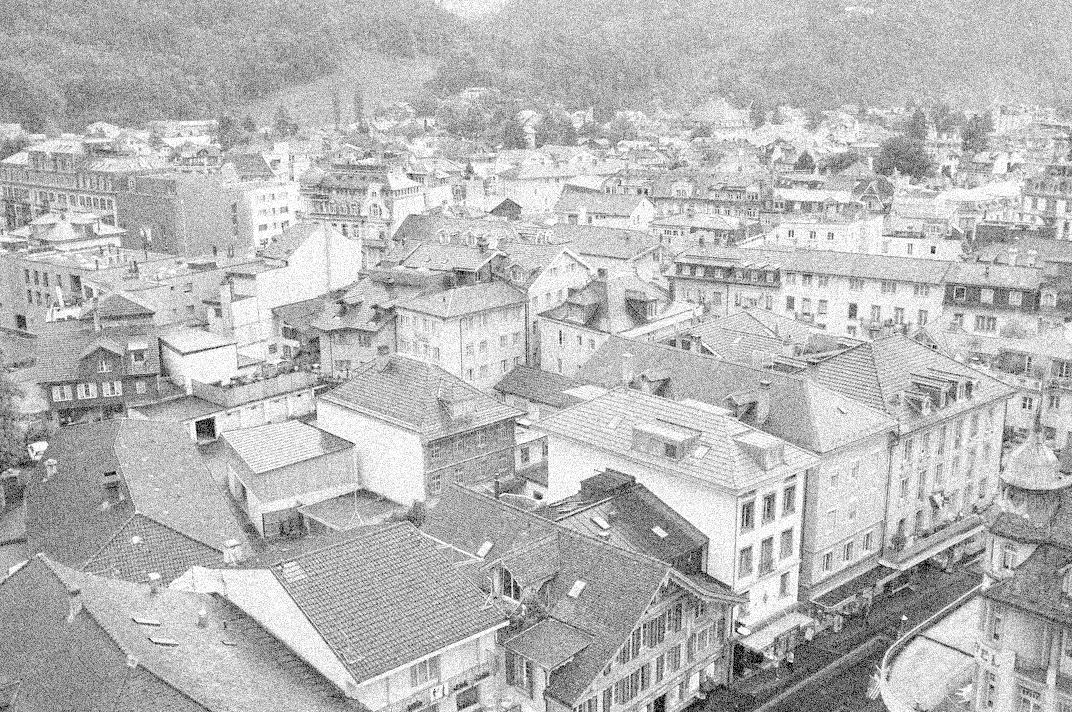
\includegraphics[width=70mm]{town_noise.png}
  \end{center}
  \caption{適用前}
  \label{fig:one}
 \end{minipage}
 \begin{minipage}{0.5\hsize}
  \begin{center}
   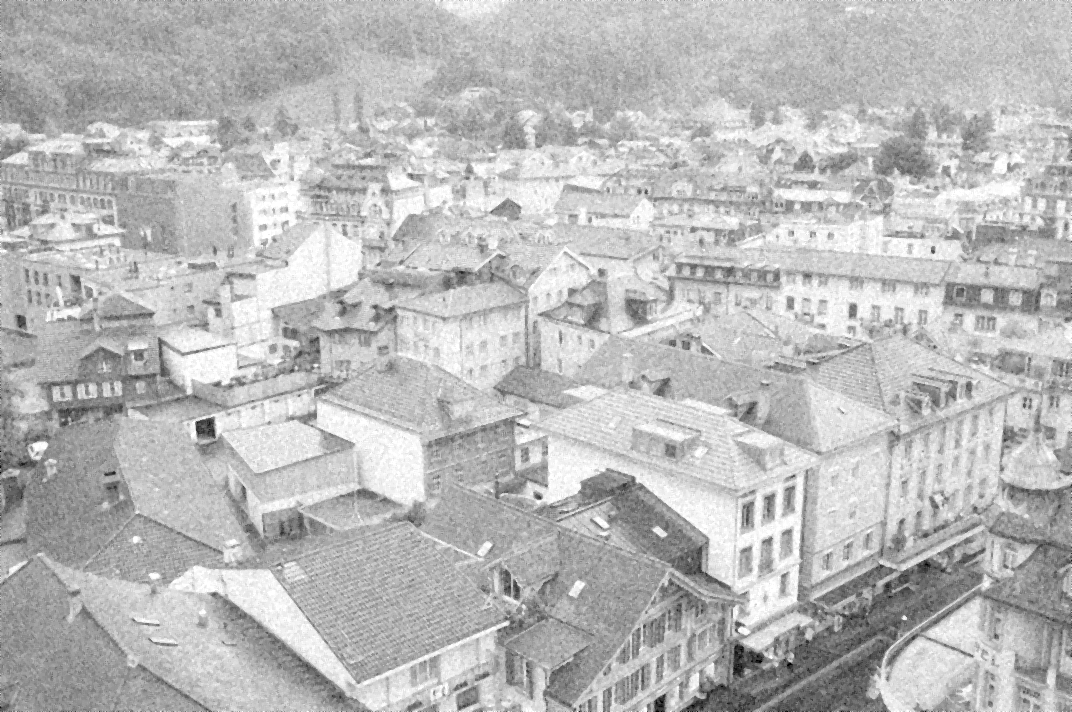
\includegraphics[width=70mm]{output_median_noise_3.png}
  \end{center}
  \caption{適用後}
  \label{fig:two}
 \end{minipage}
 \caption{ノイズ重畳画像に対してメディアンフィルタを適用(カーネルサイズ:3)}
\end{figure}

\begin{figure}[htbp]
 \begin{minipage}{0.5\hsize}
  \begin{center}
   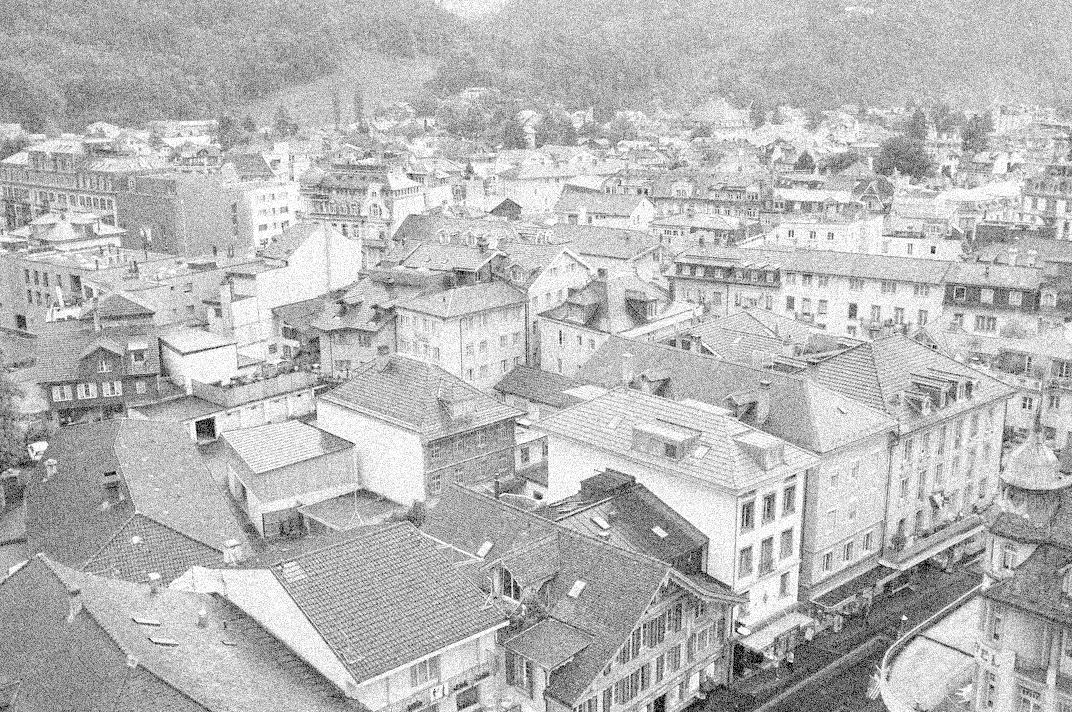
\includegraphics[width=70mm]{town_noise.png}
  \end{center}
  \caption{適用前}
  \label{fig:one}
 \end{minipage}
 \begin{minipage}{0.5\hsize}
  \begin{center}
   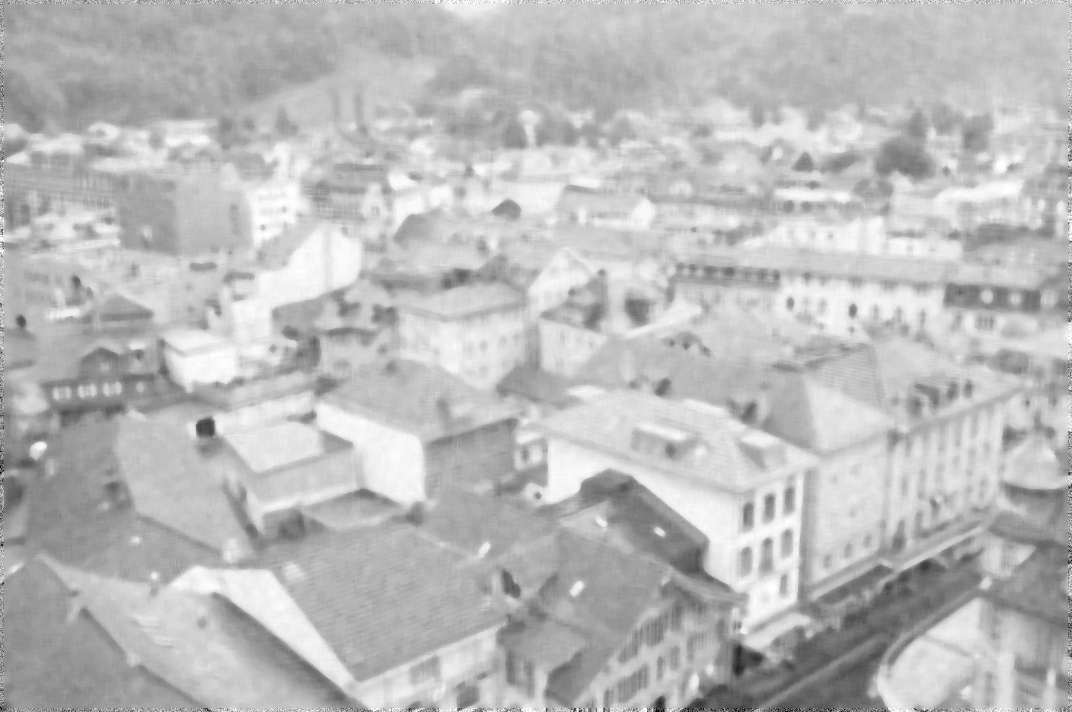
\includegraphics[width=70mm]{output_median_noise_9.png}
  \end{center}
  \caption{適用後}
  \label{fig:two}
 \end{minipage}
 \caption{ノイズ重畳画像に対してメディアンフィルタを適用(カーネルサイズ:9)}
\end{figure}

\section{考察}

加重平均フィルタでは,画像全体が均一にボケているのが確認できる.
また,カーネルサイズを大きくすると,より画像がボケていることも確認できる.

メディアンフィルタでは,同じカーネルサイズでも加重平均フィルタに比べてエッジが保存されつつ,画像がなめらかになっていることがわかる.

ラプラシアンフィルタでは,画像中のエッジが期待通り抽出できていることが確認できる.

ノイズ除去効果については,カーネルサイズ:3のときはあまり効果が得られなかったが,カーネルサイズ:9のときはかなりノイズが除去されていることがわかるが,画像自体もかなりボケてしまっている.ノイズ除去に関しては,やはりガウシアンフィルタやバイラテラルフィルタといった,より高度なフィルタを使用することが望まれる.

\section{感想}
今回,一番躓いたところは,pgmファイルを先頭から読み取っていく際に,配列を縦横逆に取り込んでいってしまったところである.一般的な感覚でコードを書くと,pgmファイルから読み取った画素値が先頭から順に縦方向に配列に格納されてしまい,後にフィルタリング処理を行う際に不都合が生じる.このバグに5時間ぐらい悩まされたのが悔しいところである.\\

\end{document}
